% =============================================================================
% Part III: The Evolution of the Science (Chapters 13--17)
% =============================================================================
\chapter{Evolution of the Research Question}\label{ch:rq_evolution}

Great empirical projects rarely end up answering the exact question they wrote on page one of their initial notebook---not because the researchers lost focus, but because early experiments reveal hidden presuppositions embedded inside the original question. Over twenty-nine days, Project CausalFade's central research question underwent six distinct formulations (\texttt{RQ1}--\texttt{RQ6}, mapped visually in Figure~\ref{fig:q_evolution}). Tracing why each formulation broke down explains the entire intellectual trajectory of the project:

\begin{enumerate}
  \item \textbf{\texttt{RQ1} --- Quantization-Induced Confounding Fallback (Oct 28 -- Nov 10, Cohorts~001--004):} \emph{Does post-training quantization (\texttt{Q4\_K\_M}, \texttt{Q2\_K}) selectively inflate an LLM's aligned-minus-conflict backdoor adjustment penalty relative to \texttt{F16}?}
  \begin{itemize}
    \item \emph{Why it proved insufficient:} Presupposed that \texttt{3B}/\texttt{7B F16} models could solve direct 4-stratum backdoor tables above chance and emit bare JSON. Instead, \texttt{3B F16} scored $33/64$ ($63/64$ \texttt{activate=1}), \texttt{7B F16} scored $17/32$ ($31/32$ \texttt{activate=1}), \texttt{Q2\_K} looped syntactically, and Cohort~002/006/007 showed that \texttt{3B Q4\_K\_M}'s real $-25\pp$ to $-31.25\pp$ drop occurred on \emph{explicit formula execution} equally across aligned and conflict items.
  \end{itemize}

  \item \textbf{\texttt{RQ2} --- Pre-Computed Evidence Source Selection and Presentation Order (Nov 10--13, Cohorts~005, 008--017):} \emph{When stratum arithmetic is removed by supplying pre-computed randomized and historical rates directly, does quantization alter preference for causal trial evidence or amplify study-order bias?}
  \begin{itemize}
    \item \emph{Why it proved insufficient:} Initially produced Cohort~016's striking $+62.5\pp$ prospective order confirmation on \texttt{Qwen2.5-7B Q4\_K\_M}, but Cohort~017 showed total failure to generalize to \texttt{14B} ($0\pp$ under $100\%$ activation), Cohort~025 showed $0\pp$ interaction on Cohort~024's semantic scaffold, and retrospective verification proved that $|\tau| < |\RD_{\mathrm{obs}}|$ allowed a source-blind smaller-gap heuristic to score $768/768$ ($100\%$).
  \end{itemize}

  \item \textbf{\texttt{RQ3} --- Component Sub-Skills vs.\ Two-Source Decision Integration (Nov 13--16, Cohorts~018--023):} \emph{Do LLMs fail two-study causal decisions because they lack causal source knowledge, because response tokens bias output polarity, or because distractor evidence disrupts single-pass integration?}
  \begin{itemize}
    \item \emph{What changed:} Cohorts~020--022 proved \texttt{Qwen2.5-7B F16} knew which study was randomized ($128/128 = 100\%$) and solved single-study RCT items ($90.6\%$--$100\%$), yet collapsed to $43.8\%$--$45.3\%$ on two-source items even when explicitly guided. Cohort~023 then revealed $<75\%$ accuracy on \emph{harmful-direction noncausal controls}, showing baseline two-table comparison itself was fragile.
  \end{itemize}

  \item \textbf{\texttt{RQ4} --- Cross-Lineage Multi-Precision Reference Gating (Nov 16--18, Cohorts~024--025.1):} \emph{Across three independent model lineages and seven GGUF precision formats, does any \texttt{F16} baseline clear directional noncausal controls, and does quantization selectively hurt causal conflict?}
  \begin{itemize}
    \item \emph{What changed:} Zero of 21 arms cleared diagnostic gates: Mistral obeyed a $100\%$ first-option policy, Llama \texttt{Q4\_K\_M} truncated on $448$ noncausal controls while leaving causal conflict untouched ($150/256$), and Qwen causal mutual information with truth was $0.031\;\text{bits}$. Quantization could no longer be the headline story when unquantized \texttt{F16} models lacked valid baseline causal sensitivity.
  \end{itemize}

  \item \textbf{\texttt{RQ5} --- Structural Graph Switching and Calculator Offloading (Nov 19--23, Cohorts~026--028):} \emph{On identical observational distributions $\Prob(W,X,Y)$, can \texttt{F16} models switch adjustment rules between confounders and mediators---especially when an exact Python calculator eliminates arithmetic error?}
  \begin{itemize}
    \item \emph{What changed:} Cohort~027 yielded $0/8$ order-robust switch fidelity across four \texttt{F16} models, and Cohort~028 proved deterministic calculation rescued noncausal named-rule controls ($+54.69\pp$ Qwen, $+34.38\pp$ Llama) while leaving causal graph rule selection near $50\%$ ($+2.34\pp$ and $-8.59\pp$).
  \end{itemize}

  \item \textbf{\texttt{RQ6} --- Shortcut-Audited Target-Population Causal Transport (\texttt{CF-TP1}, Nov 23--26, Cohort~029):} \emph{Under an exact-rational, $162$-policy shortcut-audited target-population transport protocol paired with an isomorphic weighted-scorecard control, can a model reverse and retain decisions appropriately as target subgroup composition shifts?}
  \begin{itemize}
    \item \emph{Why narrowing and reframing strengthened validity:} Far from ``moving the goalposts'' to manufacture a positive result, \texttt{RQ6} accepted a statistically inconclusive primary contrast ($\widehat{\Delta} = -3.52\pp$) while delivering a permanent methodological advance: proving how pairwise reversal/invariance decomposition separates $97.2\%$ constant-action collapse ($3/256$ causal switches) from noisy weighted aggregation ($27/256$ switches, $45/256$ false flips).
  \end{itemize}
\end{enumerate}

% =============================================================================
\chapter{The Hypothesis Ledger}\label{ch:hypothesis_ledger}

Across thirty-one cohort units, twenty distinct scientific and technical hypotheses (\texttt{H01}--\texttt{H20}) were formulated, tested, and adjudicated. Figure~\ref{fig:hyp_tree} visualizes their hierarchical branching structure and empirical verdicts, while Appendix~G (Table~\ref{tab:hypothesis_ledger}) archives the full machine-readable ledger (\texttt{evidence/hypothesis\_ledger.csv}).

\begin{figure}[htbp]
  \centering
  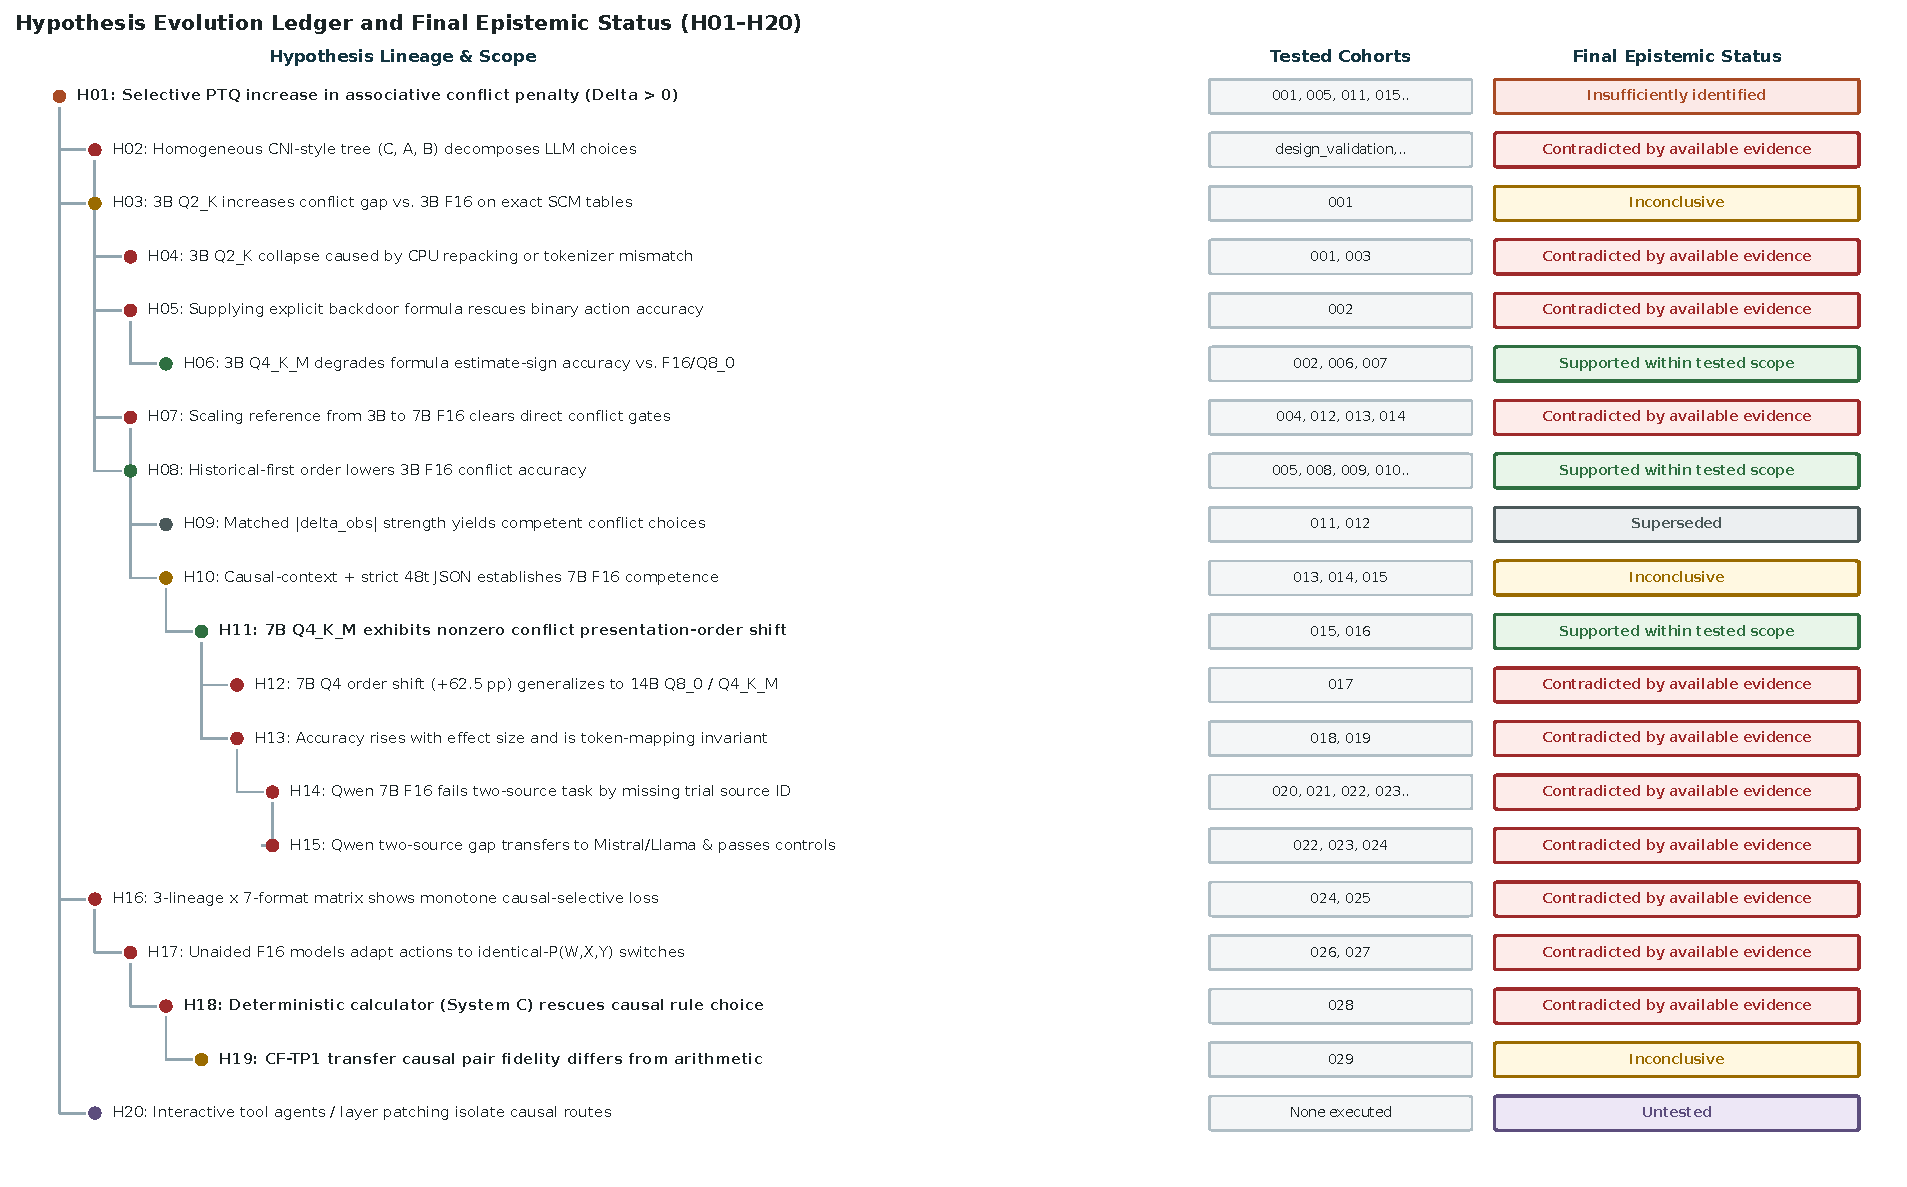
\includegraphics[width=\textwidth]{figures/fig04_hypothesis_tree.pdf}
  \caption{Hierarchical Hypothesis Tree (\texttt{H01}--\texttt{H20}) of Project CausalFade, color-coded by final evidentiary status across prospective, exploratory, and diagnostic branches.}
  \label{fig:hyp_tree}
\end{figure}

Three overarching epistemic patterns stand out across \texttt{H01}--\texttt{H20}:
\begin{enumerate}
  \item \textbf{Hypotheses Contradicted by Available Evidence ($9$ of $20$):} Including homogeneous $C/A/B$ processing-tree validity (\texttt{H02}, $-43.75\pp$ additivity residual), CPU repacking as the cause of \texttt{Q2\_K} looping (\texttt{H03}), neutral \texttt{K}/\texttt{M} symbol invariance (\texttt{H07}, $+25.8\pp$ to $+36.7\pp$ order bias), explicit source-guidance rescue (\texttt{H09}, $58/128 \to 58/128$), cross-scale 14B order generalization (\texttt{H06b}, $-4.17\pp$ and $0\pp$), order-robust confounder-vs.-mediator switching across four \texttt{F16} models (\texttt{H12}, $0/8$), and calculator rescue of causal rule selection (\texttt{H14}, $+2.34\pp$ and $-8.59\pp$).
  \item \textbf{Hypotheses Insufficiently Identified Due to Baseline Degeneracy ($4$ of $20$):} Most importantly, founding hypothesis \texttt{H01} (selective quantization inflation of causal conflict penalty) and Cohort~029's incremental causal-minus-arithmetic transport gap (\texttt{H15}, $\widehat{\Delta} = -3.52\pp$, Welch $t$ CI $[-7.77, +0.74]\pp$). Whenever the reference model or matched arithmetic baseline itself fails to execute valid decision reversals ($28.52\%$ arithmetic fidelity; $<75\%$ harmful-direction controls in Cohort~024), selective higher-order causal loss is mathematically under-identified.
  \item \textbf{Hypotheses Positively Confirmed and Replicated ($7$ of $20$):} Including \texttt{3B Q4\_K\_M}'s formula-assisted numeric ATE sign deficit (\texttt{H04}, $-25.0\pp$ in Cohort~002 and $-31.25\pp$ on fresh families in Cohort~007, spared at \texttt{Q8\_0} in Cohort~006), \texttt{3B F16}'s historical-first primacy pull (\texttt{H05}, $-21.9\pp$ to $-28.1\pp$ across Cohorts~008--011), \texttt{7B Q4\_K\_M}'s template-specific conflict-order swing (\texttt{H06a}, $+62.5\pp$ on $96$ fresh families in Cohort~016, $p = 1.24\times 10^{-37}$), Qwen's single-source vs.\ two-source component dissociation ($+48\pp$ to $+55\pp$ across Cohorts~020--023), Cohort~028's $+54.69\pp$ / $+34.38\pp$ calculator rescue on noncausal named-rule tasks, and Cohort~029's qualitative divergence between constant causal activation ($995/1{,}024$) and noisy arithmetic switching ($46/256$ switch changes, $45/256$ invariant flips).
\end{enumerate}

% =============================================================================
\chapter{The Methodological Evolution}\label{ch:method_evolution}

If CausalFade's empirical answers were predominantly negative, its methodological evolution was relentlessly constructive. Nineteen distinct methodological innovations (\texttt{M01}--\texttt{M19}, cataloged in Appendix~H, Table~\ref{tab:methodology_ledger}) were introduced, stress-tested, and either refined or retired across the archive. Figure~\ref{fig:meth_matrix} plots the exact cohort-by-methodology adoption matrix across all thirty-one cohort units.

\begin{figure}[htbp]
  \centering
  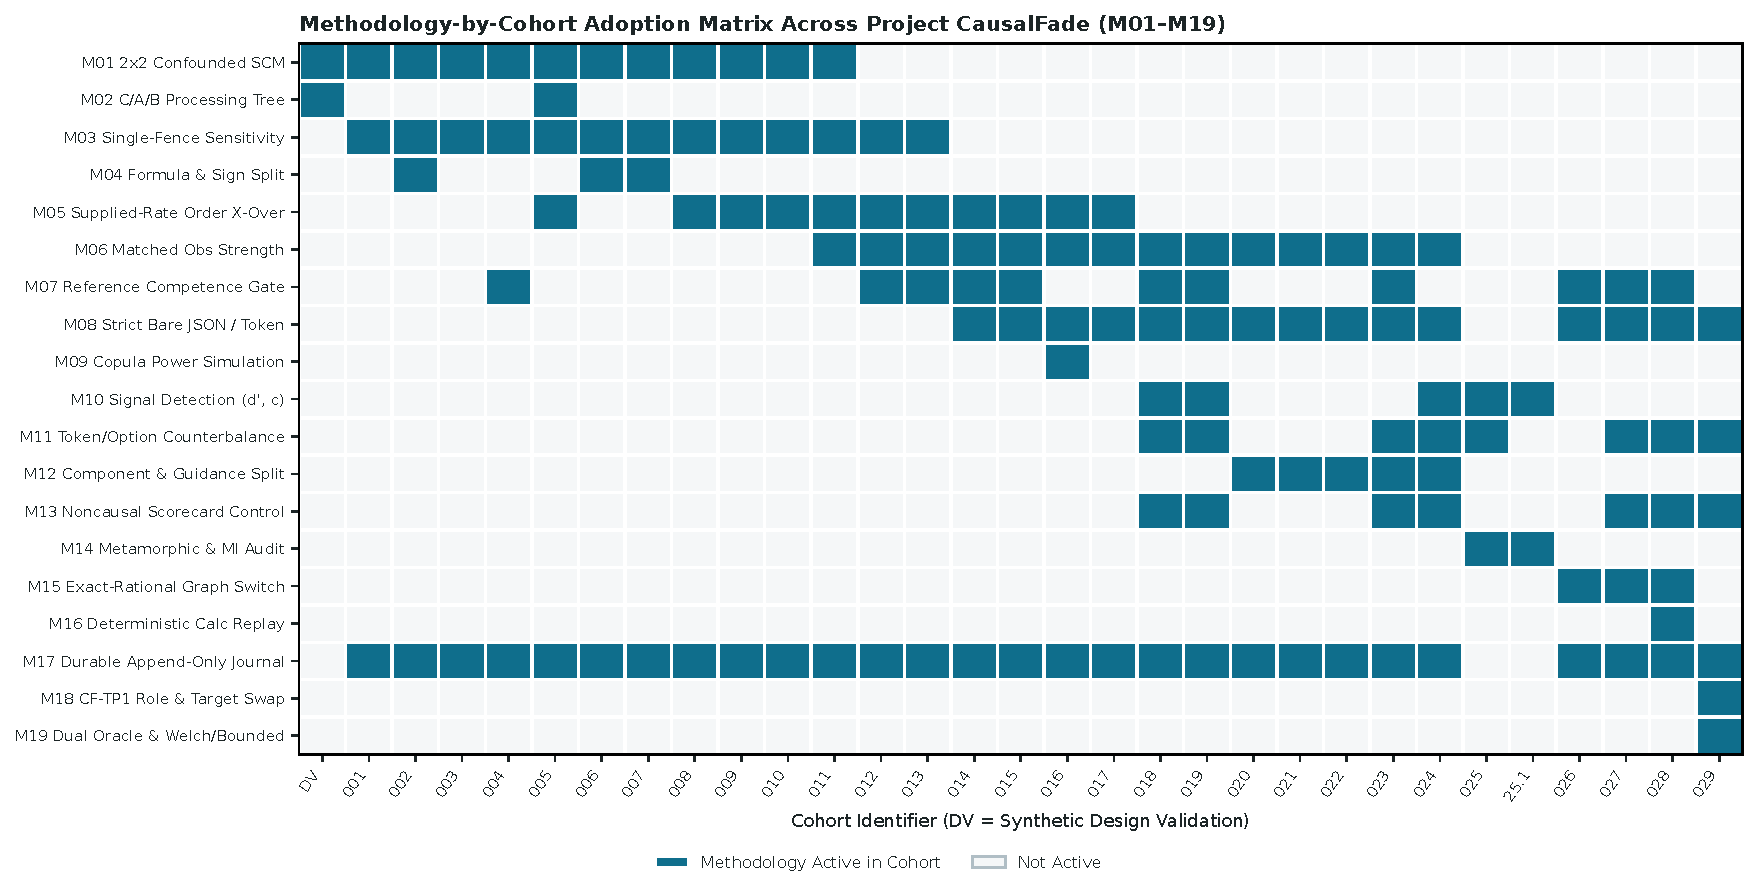
\includegraphics[width=\textwidth]{figures/fig05_methodology_cohort_matrix.pdf}
  \caption{Methodology-by-cohort evolution matrix (\texttt{M01}--\texttt{M19}) across \texttt{design\_validation} and Cohorts~001--029, tracing the retirement of $C/A/B$ trees and unmatched single-item scores in favor of reference gates, matched controls, exact-rational synthesis, shortcut audits, and pairwise fidelity.}
  \label{fig:meth_matrix}
\end{figure}

Five enduring methodological upgrades define this progression:
\begin{enumerate}
  \item \textbf{From Latent Psychometric Trees (\texttt{M02}) to Nonparametric Pairwise Transitions (\texttt{M19}):} Rather than fitting 3-parameter multinomial trees that assume cross-cell homogeneity (falsified in Cohort~005) and mimic continuous logistic models (\texttt{design\_validation}), CausalFade moved through Signal Detection Theory $(d', c)$ (\texttt{M11}, Cohort~024) to exact contrast-pair bundle scoring $F_{\mathrm{pair}} = I_0 I_1$ partitioned into required switches ($g_0 \neq g_1$) and required invariances ($g_0 = g_1$).
  \item \textbf{From Floating-Point Heuristic Worlds (\texttt{M01}, \texttt{M06}) to Exact-Rational Role-Swapped Synthesis (\texttt{M15}, \texttt{M18}):} Early NumPy floating-point generators inadvertently left magnitude fingerprints ($57\pp$ vs.\ $38\pp$ in \texttt{M01}; $|\tau| \in [6,12)\pp < |\RD_{\mathrm{obs}}| \in [38,46)\pp$ in \texttt{M06}). Cohorts~026--029 replaced floating-point sampling with exact \texttt{fractions.Fraction} arithmetic on bounded grids, verifying analytically that displayed rounded percentages preserve every true interventional inequality and role symmetry.
  \item \textbf{From Unchecked Prompts to Pre-Execution Deterministic Shortcut Audits (\texttt{M18}):} Inspired by the retrospective discovery of Cohort~016's $768/768$ smaller-gap shortcut, Cohort~029 evaluated $162$ deterministic noncausal heuristics (\texttt{policy\_audit.json}) \emph{before} freezing the fixture, guaranteeing mathematically that no source-blind or target-blind policy could exceed structural baselines.
  \item \textbf{From Uncontrolled Causal Stories to Isomorphic Noncausal Controls and Calculator Ablations (\texttt{M04}, \texttt{M10}, \texttt{M17}):} Every mature cohort paired its causal task with a structurally identical noncausal task (formula control in 002/006/007; conditional rule control in 018; PRIMARY/SECONDARY scorecard in 023--024; named \texttt{marginal}/\texttt{conditional} rule + Python calculator in 028; weighted Amber/Blue scorecard in 029).
  \item \textbf{From Ad-Hoc Runs to Pre-Declared Competence Gates and Cryptographic Journals (\texttt{M05}, \texttt{M14}, \texttt{M19}):} Pre-declared gates lawfully halted seven cohorts (004, 012, 018, 019, 026, 027, 028) before wasting compute or inflating familywise false positives on degenerate baselines, culminating in Cohort~029's SHA-256-bound append-only \texttt{events.jsonl} journal.
\end{enumerate}

% =============================================================================
\chapter{The Failures That Changed the Research}\label{ch:failures}

In textbook reconstructions of science, technical bugs and failed pilots are swept out of sight. In Project CausalFade, \textbf{failures were the primary engine of discovery}. Figure~\ref{fig:fail_timeline} maps eight specific experimental and technical failures directly to the methodological safeguards they forced into existence.

\begin{figure}[htbp]
  \centering
  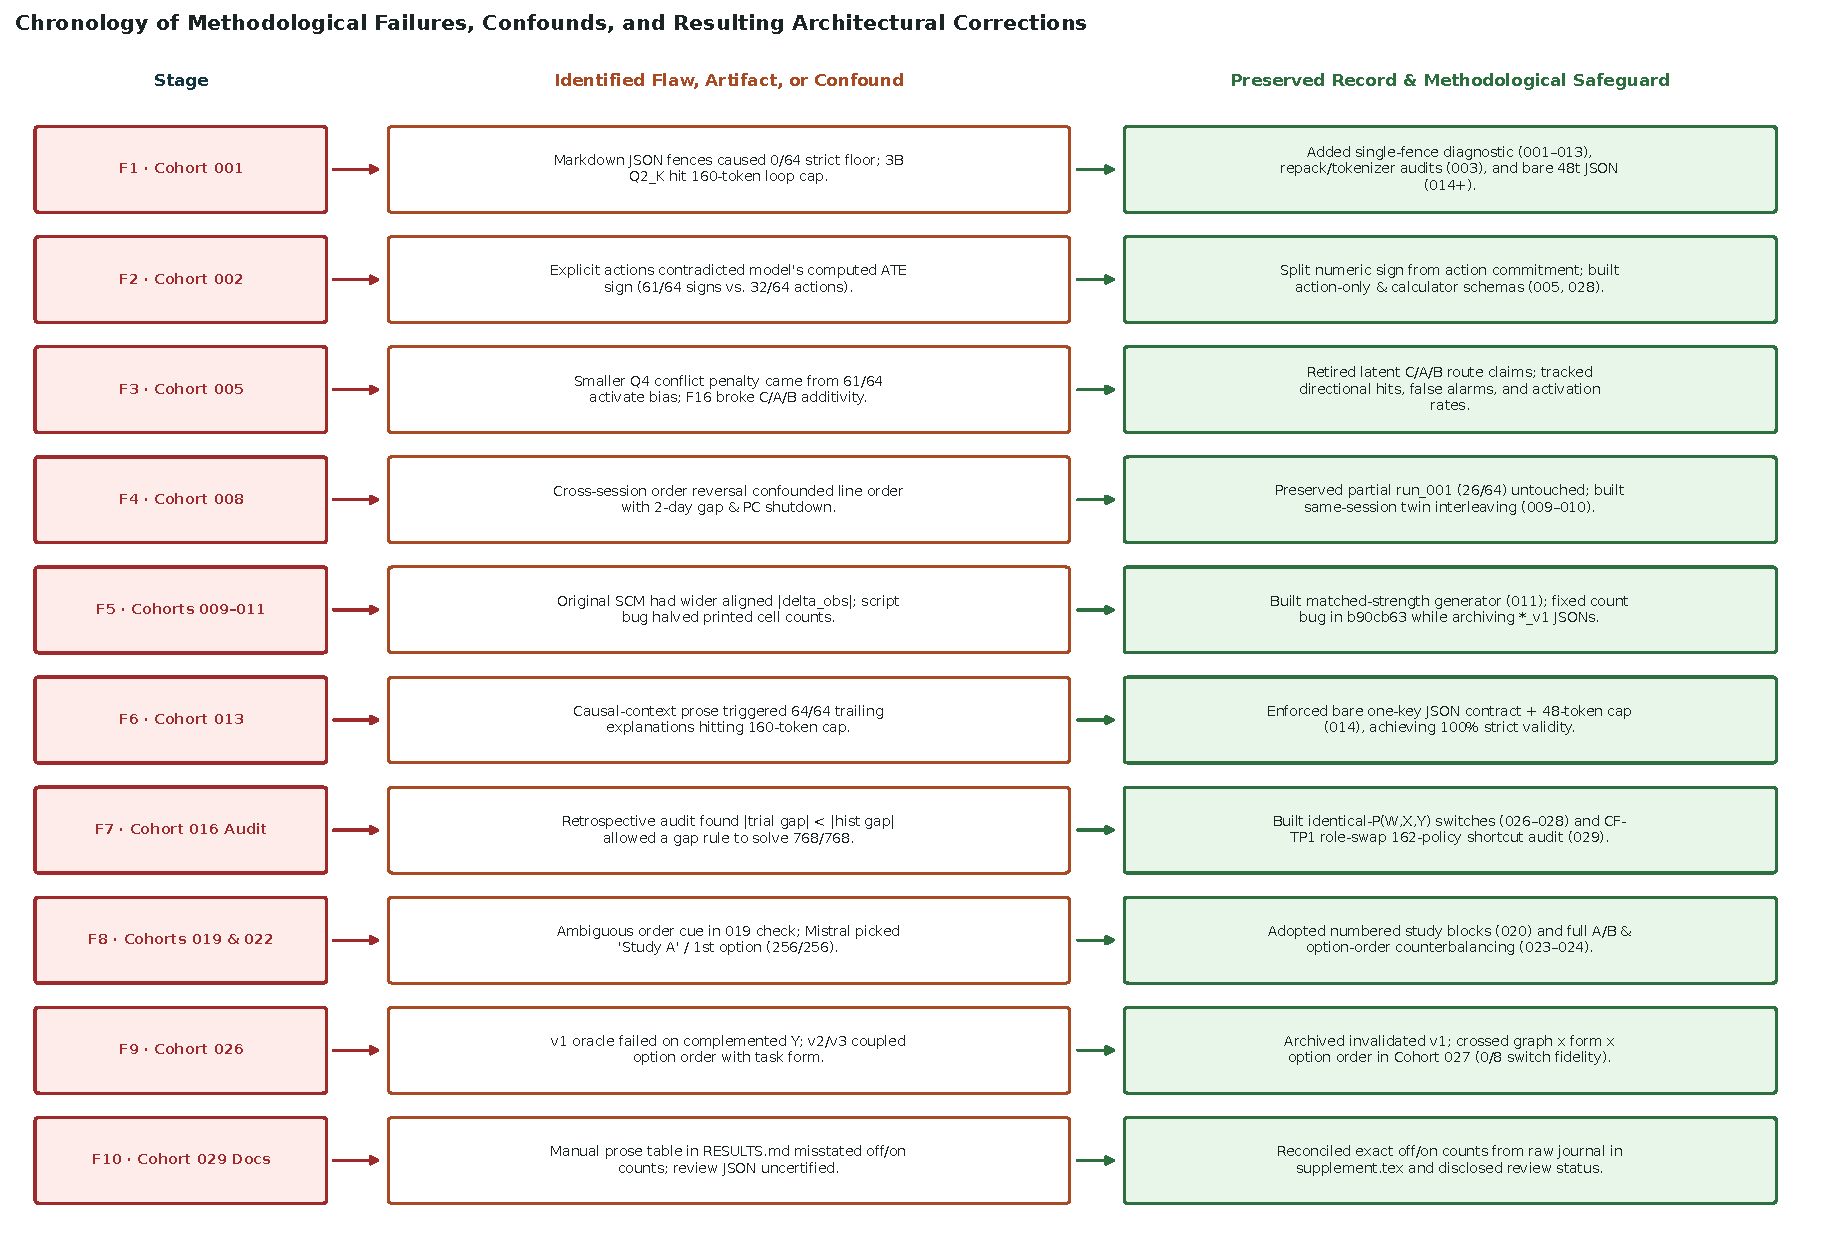
\includegraphics[width=\textwidth]{figures/fig15_failure_correction_timeline.pdf}
  \caption{Causal mapping from eight pivotal experimental, parser, oracle, and construct-validity failures across CausalFade to the permanent methodological and engineering safeguards they produced.}
  \label{fig:fail_timeline}
\end{figure}

\begin{enumerate}
  \item \textbf{Failure 1 --- Cohort 001's $0/64$ Markdown Fence Wipeout:} \texttt{Qwen2.5-3B F16} emitted valid JSON wrapped in \texttt{```json} fences on $64/64$ items, scoring $0\%$ under naive \texttt{json.loads}. \emph{Correction:} Dual strict/fence-stripped reporting (Cohorts~001--012) followed by explicit negative prompt constraints (\emph{``Do not include a Markdown fence, explanation, or any other text''}) achieving $100\%$ bare-JSON compliance from Cohort~014 onward.
  \item \textbf{Failure 2 --- Cohort 002's $63/64 \to 0/64$ Action Flip and Numeric-Action Split:} Supplying the backdoor formula caused \texttt{3B F16} to compute $61/64$ right ATE signs while flipping explicit \texttt{activate} choices from $63/64$ ones to $0/64$ ones! \emph{Correction:} Separated latent numeric estimation from binary decision commitment and moved to single-key action schemas.
  \item \textbf{Failure 3 --- Cohort 005's $-43.75\pp$ $C/A/B$ Additivity Violation and Inverted Penalty:} \texttt{Q4\_K\_M} reduced the conflict penalty by $-43.75\pp$ purely via $61/64$ constant activation, while \texttt{F16} broke tree additivity by $-43.75\pp$. \emph{Correction:} Immediate retirement of $C/A/B$ tree claims (\texttt{D05}) and mandatory reporting of directional activation rates alongside accuracy.
  \item \textbf{Failure 4 --- Cohort 009--011's Display-Count Halving Bug and Cohort 017's Missing-NumPy Crash:} Post-run scripts divided displayed raw counts by $2$ (Cohorts~009--011) and crashed in an unattended shell lacking NumPy (Cohort~017). \emph{Correction:} Archived buggy \texttt{v1} files transparently alongside fixed analyzers (commit \texttt{b90cb63}), added zero-variance Student-$t$ guards, and built zero-dependency/pinned verification scripts.
  \item \textbf{Failure 5 --- Cohort 013's $64/64$ Post-JSON Causal Verbosity Spillover:} Mentioning causal confounding triggered \texttt{7B F16} to append explanatory paragraphs after its JSON block until hitting the 160-token cap. \emph{Correction:} Tightened output contracts and token budgets (\texttt{max\_tokens=48}), solving strict validity ($128/128$ in Cohort~014).
  \item \textbf{Failure 6 --- Cohort 016's $768/768$ Source-Blind Smaller-Gap Shortcut:} Retrospective audit revealed $|\tau| \in [6,12)\pp < |\RD_{\mathrm{obs}}| \in [38,46)\pp$ everywhere in Cohorts~011--017. \emph{Correction:} Role-swapped symmetric table generation and pre-run $162$-policy deterministic shortcut audits in Cohort~029.
  \item \textbf{Failure 7 --- Cohort 024's $448$ \texttt{Llama Q4\_K\_M} Control Truncations and $256/256$ \texttt{Mistral F16} First-Option Collapse:} Proved that quantization can selectively break formatting on \emph{control} prompts while sparing causal prompts, and that unquantized 7B models can obey $100\%$ positional heuristics. \emph{Correction:} Strict option-order counterbalancing and scheduled-denominator accounting.
  \item \textbf{Failure 8 --- Cohort 026's v1 $Y$-Complement Oracle Bug, v2 Period Failure (\texttt{"X=1."}), and v3 Option-Order Mirage ($6/8 \to 0/8$):} Showed how a subtle oracle sign bug, a single trailing period, and uncrossed option order could manufacture false negatives and false positives within the same day. \emph{Correction:} Preserved \texttt{invalidated\_pilot\_qwen\_v1}, enforced exact-rational sign checks, and fully crossed forward/reverse option order in Cohort~027 (proving true switch fidelity was $0/8$).
\end{enumerate}

% =============================================================================
\chapter{The Turning Points}\label{ch:turning_points}

Stepping back across all 320 Git commits and 30 decisions (\texttt{D01}--\texttt{D30}, Appendix~I), six decisive turning points shaped CausalFade into its final scientific form:

\begin{enumerate}
  \item \textbf{Turning Point 1 (Oct 28 -- Nov 1, commits \texttt{4e2fe4f}--\texttt{6ab18d2}): Behavioral Scoping and Pre-LLM Synthetic Falsification.} Refusing mechanistic ``circuit severing'' claims upfront and proving symmetric logistic equivalence of the $C/A/B$ tree before running Cohort~001 established an ethos of mathematical skepticism.
  \item \textbf{Turning Point 2 (Nov 10, commits \texttt{01c7590}--\texttt{4e90b24}, Cohorts~004--005): Reference Competence Gates and Retirement of $C/A/B$ Trees.} Establishing the rule that quantized runs are uninterpretable when \texttt{F16} fails competence gates prevented twenty cohorts of spurious noise chasing.
  \item \textbf{Turning Point 3 (Nov 12--13, commits \texttt{eb53578}--\texttt{caf5b1d}, Cohorts~016--017): The High-Water Mark of Order Sensitivity and Its Immediate Cross-Scale Failure.} Watching a $t(95)=21.10$ ($p=1.24\times 10^{-37}$) 7B effect vanish completely at 14B taught the project that statistical significance within one template is never equivalent to construct validity or model-family generality.
  \item \textbf{Turning Point 4 (Nov 14--16, commits \texttt{737c945}--\texttt{4aff668}, Cohorts~020--023): Component Competence vs.\ Action Collapse and Harmful-Direction Control Failure.} Discovering $128/128$ governing-source recognition alongside $58/128$ guided decision-making---and $<75\%$ harmful-direction noncausal controls---reframed the entire problem around cue integration and matched baselines.
  \item \textbf{Turning Point 5 (Nov 16--23, commits \texttt{6193357}--\texttt{ac6ed58}, Cohorts~024--028): Closing the Quantization-First Era and Isolating Causal Rule Selection via Python Calculation.} Cohort~024's 21-arm matrix ($0/21$ gates passed) ended hopes of a selective PTQ causal story, while Cohort~028's calculator ablation ($+54.7\pp$ noncausal vs.\ $+2.3\pp$ causal) proved causal adjustment selection fails independently of arithmetic.
  \item \textbf{Turning Point 6 (Nov 23--26, commits \texttt{76206c2}--\texttt{b737153}, Cohort~029 \& \texttt{manuscript/}): Target-Population Transport (\texttt{CF-TP1}) and Retrospective Shortcut Transparency.} Rather than burying Cohort~016's shortcut flaw or spinning Cohort~029's $-3.52\pp$ null, the final framework turned both into lasting methodological contributions.
\end{enumerate}
